\jxhj{%教学后记
	}
\skrq{%授课日期
	2017年9月14日 4-5节}
\ktmq{%课题名称
	基本指令(一) }
\jxmb{%教学目标,每行前面要加 \item
	\item 掌握G1与G0的区别。
    \item 掌握G2/G3的基本应用。
    \item 掌握编写数控程序的基本思路。
    \item 了解数控常见指令。}
\jxzd{%教学重点,每行前面要加 \item
	\item 掌握G1与G0的区别;
	\item 掌握G2/G3的基本应用;}
\jxnd{%教学难点,每行前面要加 \item
	\item 掌握G2/G3的基本应用;}
\jjff{%教学方法
	通过讲述、举例、演示法来说明;}

\makeshouye %制作教案首页

%%%%教学内容
\subsection{组织教学}
\begin{enumerate}[1、]
	\item 集中学生注意力;
	\item 清查学生人数;
	\item 维持课堂纪律;
\end{enumerate}
\subsection{复习导入及主要内容}
\begin{enumerate}[1、]
\item 案例分析;
\item 指令讲解;
\item 编写程序;
\item 编写程序的基本思路。
\end{enumerate}


\textbf{G0与G1的区别}

\begin{enumerate}[1、]
\item 指令格式不同:G1使用前必须用F设定进给速度,G0的速度与F无关 
\item 运动轨迹不同:G0为快速定位,其路径可能为直线,也可能为折线。G1为直线插补,其路径为直线。
\item 进给速度不同:G0的速度由机床参数及快速倍率决定,档位少。G1的速度由F及进给倍率决定,可调档位多。
\item 功能用途不同:G0用于加工前的定位及加工后的提刀,G1用于车削加工
\end{enumerate}
注意:

新学的同学用G1 F2000 代替 G0 (可控与不可控)

不要三坐标编程,定位时,先提刀,再定位。

\subsection{教学内容及过程}
\subsubsection{案例分析}

在数控铣床或加工中心上加工如图\ref{fig:4-1}所示的零件,试完成程序的编写,已知毛坯为 $\Phi$ 110*30。

\begin{figure}[h]
    \centering
    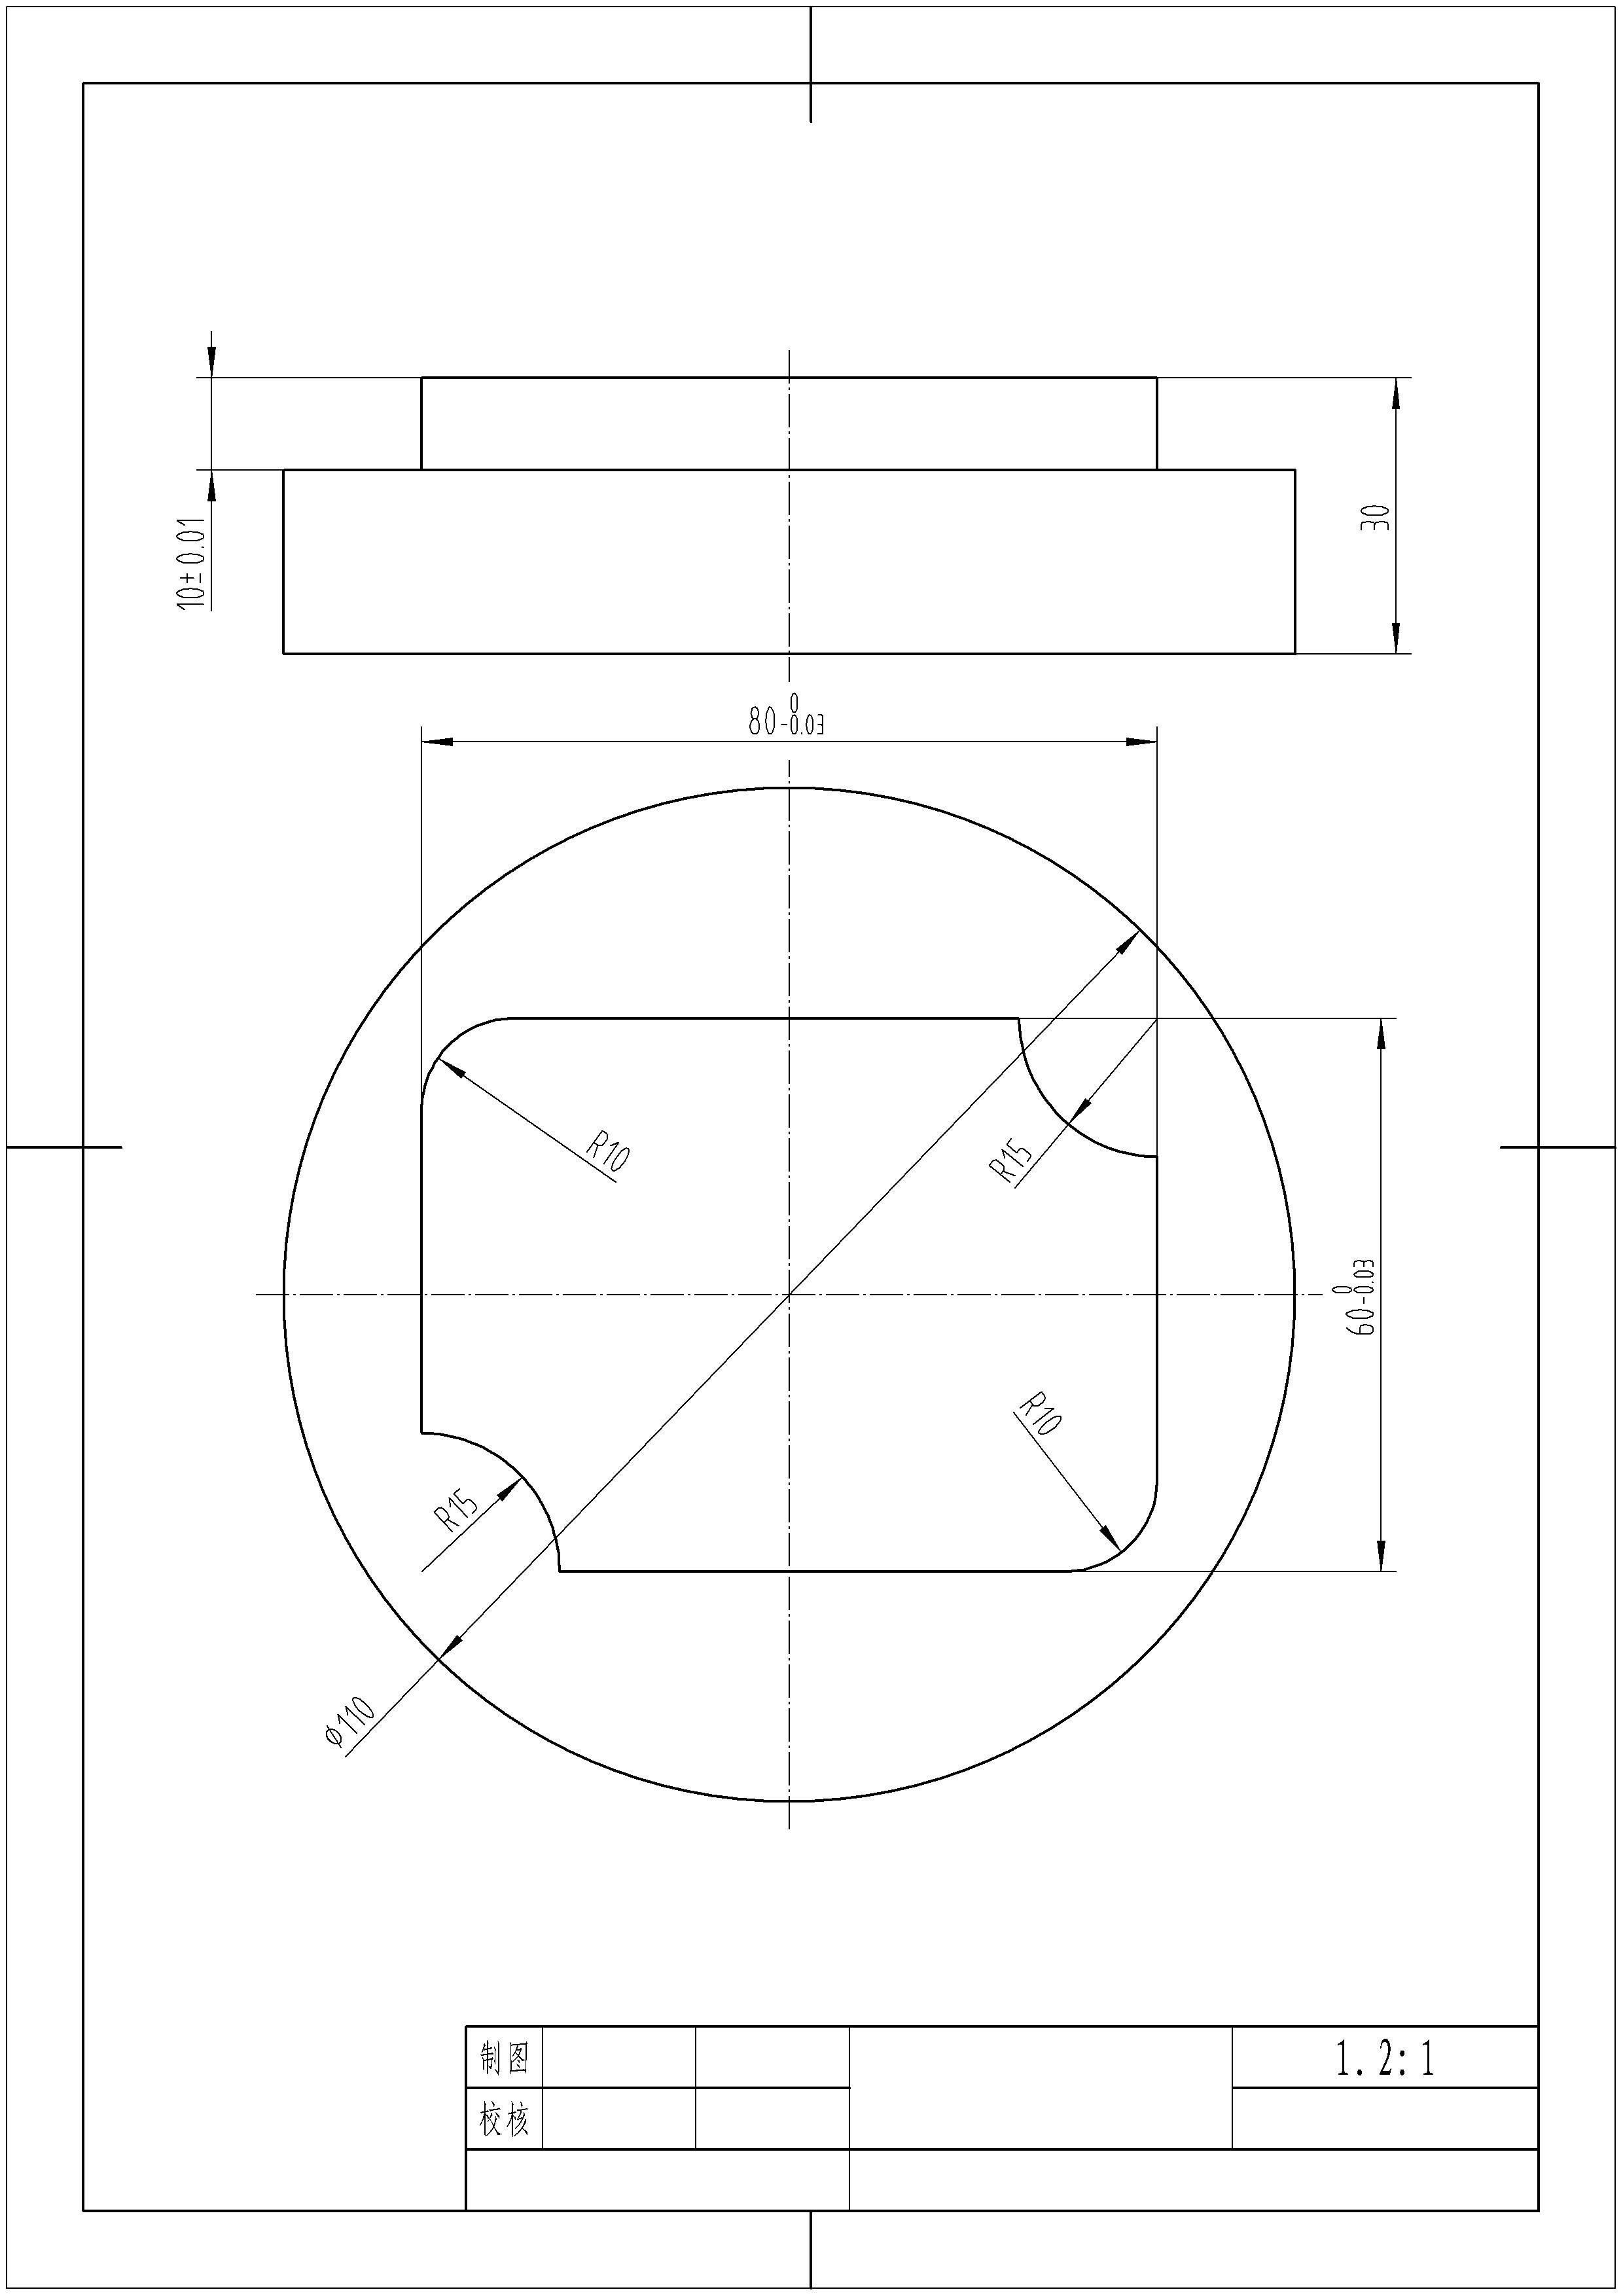
\includegraphics[width=0.8\linewidth,trim=50 150 50 100,clip]{data/image/4-1.jpg}
    \caption{}
    \label{fig:4-1}
\end{figure}

\begin{enumerate}[1、]
    \item 图样分析;
    \item 确定加工内容;
    \item 确定装夹及工件坐标系;
    \item 确定刀具及切削用量;
    \item 确定工序及走刀路线;
    \item 计算点坐标;
    \item 编写程序单。
\end{enumerate}

\subsubsection{G02/G03指令(只讲R编程)}

常见的圆弧标注—— 半径

起点——终点——半径

圆弧插补指令:

1、[格式]
XpYp平面的圆弧   
G17  G2/G3  X\_ Y\_ R\_ F\_
ZpXp平面的圆弧   
G18 G2/G3 Z X R F 
YpZp平面的圆弧   
G19 G2/G3 Y Z R F
对于我们学校的一般用G17平面

指令格式的说明

G17	指定圆弧在XpYp平面

G18	指定圆弧在XpZp平面

G19	指定圆弧在YpZp平面

G02	顺时针方向圆弧插补(CW)

G03	逆时针方向圆弧插补(CCW)

Xp\_\_	X轴或平行于X轴的指令值(由参数No.1022设定)

Yp\_\_	Y轴或平行于Y轴的指令值(由参数No.1022设定)

Zp\_\_	Z轴或平行于Z轴的指令值(由参数No.1022设定)

R\_\_	圆弧半径指定的带符号的圆弧半径

F\_\_	沿圆弧的进给率 



2、圆弧插补的方向

在XpYp平面(ZpXp平面或YpZp平面)“顺时针方向”(G02)和“逆时针方向”(G03)是从笛卡尔坐标系的Zp轴(Yp轴或Xp轴)去看正负方向来决定的,

3、目标点坐标

用位址Xp,Yp,Zp指定的圆弧的端点是根据G90还是G91来表达是绝对值还是相对值。

对于相对值, 终点的距离要从指定圆弧的起点来看。

4、举例:

A-B   G91   G90 

……   ( 学生练习)




\subsubsection{编写程序的基本思路}
程序初始化(安全保护)--------辅助准备(换刀,主轴启动,切削液开)--------定位到起刀点--------快速下刀--------工进下刀--------走加工轮廓--------提刀---------快速提刀到安全平面-------程序结束(换刀,主轴停止,切削液关,程序返回等)
\subsection{课堂小结}
\begin{enumerate}[1、]
\item 案例分析;
\item 指令讲解;
\item 编写程序;
\item 编写程序的基本思路。
\end{enumerate}
\vfill
\subsection{布置作业}
\begin{enumerate}[1、]
	\item 自定尺寸,编写加工一个矩形外形的程序?
\end{enumerate}
\vfill